%-*-coding: utf-8-*-

\graphicspath{ {images/} }

\startrelatedwork

\chapter{Обзор предметной области} \label{chapter1}
В данной главе проводится обзор предметной области.
Дается объяснение технологии <<блокчейн>>, понятия алгоритма консенсуса, транзакциях и
криптографических примитивов.
Далее следует рассмотрение существующих решений и описание их недостатков.

\section{Технология блокчейн}

Технология блокчейн, от английского blockchain, дословно переводится  как "цепочка блоков".

Блок хранит в себе данные, а также ссылку на предыдущий блок. 
Блоки образуют бесконечную последовательность, которая имеет начало, но не имеет конца.
Первый блок в блокчейне называется \textit{генезис блоком} (genesis block).

По сути, блокченй представляет односвязный список, где каждый элемент знает ссылку на предыдущий. 
Однако, особенностью данного списка является то,  что в качестве ссылки на предыдущий блок 
используется хэш криптографически стойкой хэш-функции содержимого предыдущего блока, 
которое включает как его данные, так и ссылку на предыдущий блок. 
Поэтому даже при малейшей попытке заменить содержимое блока, 
поменяется значение хэш-функции его данных и ссылка на него от последующего блока будет недействительна.
Нахождение двух блоков с разным содержанием и одинаковым значением хэш-функции является  задачей, требующей экспоненциального количества вычислений. 
Таким образом, хэш последнего блока в цепочке является доказательством данной цепочки, то есть легко проверить что данный хэш соответствует цепочке, но создать другую цепочку с таким же хэшом является вычислительно сложной задачей. Данная особенность ключевая, и  является одной из основных для обеспечения безопасности в криптовалютах использующих технологию блокчейн.

\begin{figure}[h]
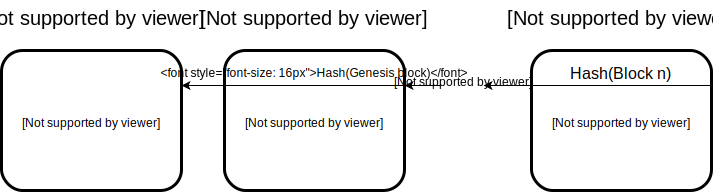
\includegraphics[scale=0.6]{Blockchain_Scheme}
\caption{\textbf{Схема блокчейна}}
\label{fig:blockchain}
\end{figure}

На Рисунке \ref{fig:blockchain} обозначено схематиченое представление блокчейна.

Будем называть описанную структуру ~--- блокчейн.

\section{Алгоритм достижения консенсуса}
Исследование в области распределенных систем началось задолго до появление криптовалют, и насчитывает 30 лет исследования и разработки.
Алгоритмы достижения консенсуса между несколькими участниками ~--- являются одной из популярных задач в этой области.
Формально, класс таких алгоритмов можно описать следующим образом:
\par \textit{
Имеется $n$ участников, между которыми установлены каналы связи. Каждый участник знает некоторое число $x$ (у каждого свое).
После некоторой коммуникации по каналам связи они хотят получить некоторое число $c$ (общее для всех),  равное одному из чисел $x$.
}

В рамках данной работы нас будут интересовать алгоритмы, которые предоставляют \textit{отказоустойчивость к Византийским ошибкам} (BFT)\cite{Lamport:1982}.
Византийская ошибка ~--- это ошибка при которой участник может отправлять любые данные по каналу связи, в том числе участник может препятствовать достижению консенсуса.
Впервые задача BFT и ее решения были описаны в работе Лампорта от 1982 года\cite{Lamport:1982}. 
В данной статье Лампорт также доказал, что не существует алгоритма, который приводит менее $3f+1$ участников в консенсусу, если среди них имеется $f$  византийских участников.
Иными словами, в алгоритме в котором участвуют $n$ участников менее $\ceil{\frac{n}{3}}$ могут быть византийскими.

Несмотря на то, что работа Лампорта имела важное теоретическое значение, предложенные в ней алгоритмы требовали экспоненциального количества сообщений между участниками, 
и едва ли могли применяться на практике для больших $n$. Поэтому в 1999 году был разработан алгоритм PBFT (Practical BFT)\cite{pbft},  в рамках которого отправляется $O(n^2)$  сообщений.

Хотя после разработки PBFT было предложено множество его улучшений \cite{qu, hq, Zyzzyva}, все они предполагали \textit{эксклюзивную} (permissioned) модель сети, 
в которой участники были заранее известны и не менялись со временем. Другая альтернатива ~--- \textit{инклюзивная} (permissionless) модель, в которой участники
неизвестны заранее и могут меняться со временем. Инклюзивная модель в большей степени подходит для консенсус алгоритмов в криптовалютах. Одним из самых известных инклюзивных алгоритмов является Nakamoto consensus\cite{nakamoto}, на основе которого построена криптовалюта Bitcoin. Nakamoto consensus и некоторые другие инклюзивные алгоритмы будут рассмотрены подробнее в следующих разделах данной главы.

\section{Транзакции и хранилище} \label{sec:tx}
Основной функционал в криптовалюте ~--- это возможность переводить другим участникам системы средства, а также получать средства на свой счет.
Рассмотрим один из способов реализации данного функционала,
в том числе, как хранится информация о счетах и как производится перевод средств между ними.

У каждого участника системы имеется \textit{адрес}, на котором хранятся его \textit{токены}, токены
являются аналогом фиатной валюты, например рубля или доллара. Количество токенов участника на его адресе будем называть \textit{балансом}. Токены между адресами пересылаются с помощью \textit{транзакции}. Транзакция ~--- это подтвержденное криптографической подписью сообщение, которое указывает с каких и на какие адреса отправлять и получать токены, а также количество токенов.

Вся информация о балансах хранится в базе данных, которую в рамках данной работы носит название \textit{хранилищем}.
Данная база данных может быть распределенной, тогда части ее будут храниться на устройствах участников системы. 
Такой подход называется шардирование (от английского sharding). 
Другой, более простой подход, состоит в том, что копия этой базы данных хранится у каждого участника системы.
В данной работе будет использоваться данный более простой подход.

Обозначим через $\boldsymbol{\sigma}$ отображение из адреса в состояние адреса. Тогда для адреса $a$ в $\boldsymbol{\sigma}[a]$ содержится:
\begin{itemize}
\item balance ~--- целая величина, количество токенов принадлежащих адресу $a$
\item nonce  ~--- целая величина, количество транзакций отправленных с этого адреса
\end{itemize}

nonce хранится для того, чтобы предотвратить двойную трату (double spending)\cite{double-spending}.

\noindent Транзакция содержит следующие данные:
\begin{itemize}
\item $s$ ~--- адрес отправителя
\item $r$ ~--- адрес получателя
\item $n$ ~--- nonce адрес отправителя в момент создания транзакции
\item $amount$ ~--- количество переводимых токенов
\item $pk$ ~--- публичный ключ отправителя (sender)
\item $sig$ ~--- подпись кортежа $(s, r, amount, n)$, сделанная с помощью секретного ключа $s$
\end{itemize}

\noindent Таким образом, каждый участник системы может проверить, что подпись действительно сделана с помощью секретного ключа, соответствующего публичному ключу pk. Попытка подделать кортеж $(s, r, amount, n)$, чтобы подпись осталась такой же, является NP полной задачей.

После того как участник системы получает транзакцию $t$, он проверяет, что выполняются следующие условия:
\begin{itemize}
\item $\boldsymbol{\sigma}[s].balance \ge t.amount$ ~--- отправитель имеет достаточное количество токенов
\item $\boldsymbol{\sigma}[s].nonce = t.n$ ~--- nonce транзакции совпадает с хранимым в хранилище
\item $verifySignature(t.sig, t.pk, (t.s, t.r, t.amount, t.n))$ ~--- подпись в транзакции корректна
\end{itemize}

Если все вышеописанные условия выполняются, то участник обновляет локальную копию хранилища следующим образом:

$\boldsymbol{\sigma}[s].balance = \boldsymbol{\sigma}[s].balance - t.amount$

$\boldsymbol{\sigma}[r].balance = \boldsymbol{\sigma}[r].balance + t.amount$

$\boldsymbol{\sigma}[s].nonce = \boldsymbol{\sigma}[s].nonce + 1$\\
Все данные изменения должны проводиться атомарно, чтобы избежать неконсистентного состояния хранилища.

%\subsection{Хранилище на основе списка непотраченых выходов}

%\section{Криптографические примитивы}

\section{Существующие криптовалюты и решения}

\subsection{Bitcoin и Bitcoin-NG}
Как уже было отмечено ранее, Bitcoin использует инклюзивный алгоритм консенсуса, который подробно описано в \cite{nakamoto}. Данный алгоритм состоит из следующих основных этапов.
Каждый участник поддерживает актуальные блокчейн и хранилище. Получая транзакции, участник формирует блок, в котором содержатся данные транзакции и ссылка на предыдущий блок. Далее участник, который называется \textit{майнер}, пытается найти некоторое целое значение $\phi$, которе будучи захэшированным вместе с хэшем содержимого созданного блока, даст значение хэш функции с определенным количеством нулей, которое называется \textit{цель} (target), подобно тому, как описано в работе \cite{hashcash}. Найдя данное значение, участник отправляет блок другим участникам, которые проверяют, что данное значение действительно удовлетворяет заданной цели, которая известна всем участникам, а также транзакции удовлетворяют условиям описанным в разделе \ref{sec:tx}. Для хэширования используется криптографически стойкой хэш функция, например SHA256 или SHA512 \cite{sha-2}.
Выпущенные блоки формируются в цепочку, которая является доказательством корректности транзакций. Алгоритмы консенсуса в основе которых лежит вычисление какой-то сложной функции для доказательства, называются  алгоритмы консенсуса на основе \textit{доказательства выполненной работы}\cite{pow}.

Цель меняется со временем, и зависит от скорости выпуска блоков. Она адаптируется таким образом, чтобы время нахождение нужного значения $\phi$  приблизительно равнялось 10 минутам. Вычисление цели подробно описано в оригинальной статье \cite{nakamoto} и рассмотрение этого вычисления не столь важно для данной работы, более важно то, что данная величина в 10 минут является ключевой, и не может быть уменьшена без потерь гарантий безопасности.

При возникновении \textit{вилки} (fork), то есть альтернативной цепочки, которая также являются продолжением блокчейна, участники выбирают наидлиннейшую корректную из цепочек. Однако, византийский участник может выбрать цепочку, которая не является корректной, в которой например содержатся транзакции, которые производят двойную трату. Данный алгоритм устойчив к византийским участникам, если их суммарная вычислительная мощность не превосходит $p$ \% вычислительной мощности всех участников системы. В оригинальной статье, $p$ заявлялось равным 50, однако дальнейшие исследования показали, что существуют атаки, которые нарушают корректность алгоритма даже при $p=25$ \cite{DBLP:journals/corr/EyalS13}.

Чтобы считаться транзакцию \textit{подтвержденной}, отправивший ее участник сети должен дождаться $O(\lambda)$  блоков после блока, в который она попала. Иначе, блок с данной транзакцией может быть \textit{откачен} (rollback), из-за возникшей вилки. Считается, что при $\lambda=6$ вероятность достаточна мала, чтобы считать отмену блоков возможной.\vspace{10pt}

Резюмируя все вышесказанное, Bitcoin имеет две основные проблемы:
\begin{enumerate}
\item большое время попадания транзакции в блок, которое равно 10 минутам. Как следствие ~--- маленькая пропускная способность;
\item время подтверждения транзакции равно 60 минутам.
\end{enumerate} \vspace{10pt}

Bitcoin-NG \cite{bitcoin-ng} является усовершенствованием Bitcoin и решает первую проблему. В предложенном в 2016 году алгоритме майнер, нашедший число $\phi$,  получает право создавать \textit{микроблоки}, в которых будут находиться транзакции. Выпуск микроблоков происходит намного чаще основных блоков ~--- раз в 10 секунд. Данное решение значительно увеличивает скорость обработки транзакций, а также уменьшает размер блоков.
Однако, предложенный алгоритм все еще страдает от второй проблемы ~--- время подтверждения все еще равно 60 минутам.

Слишком долгое время подтверждения транзакции ~--- это не только проблема Bitcoin, но и многих других криптовалют, которые предоставляют \textit{консистентность в конечном счете}, то есть в которых последние $O(\lambda)$ блоков могут быть откачены. Данная проблема присуща таким известным проектам как Etherium\cite{buterin2014ethereum} и Cardano \cite{cardano}.

Данная проблема была формализована в статье Hybrid Consensus \cite{hybrid-consensus} теоремой, следствие из которой звучит как: 
\par \textit{не существует отзывчивого протокола, который бы оставался безопасным при доле нечестных участников превышающей $\frac{1}{3}$ от общего числа}.

Отдельного внимания заслуживает термин \textit{отзывчивость} протокола. Неформально он означает, что подтверждение транзакции ограничено некоторой величиной $O(\delta)$, где $\delta$ ~--- это время распространения транзакции по сети. Он будет введен формально в следующей главе.
 
Данное следствие распространяется как на эксклюзивные, так и на инклюзивные протоколы. 
В частности, оно означает, что Bitcoin и подобные протоколы, не могут обрабатывать транзакции с временем подтверждения $O(\delta)$.

\subsection{Алгоритм XFT}
В работе\cite{DBLP:journals/corr/LiuCQV15}, предложенной  Shengyun Liu, описывается решение, которое основывается на предположении, что византийская ошибка ~--- это слишком <<сильная>> модель для злоумышленника. Авторы работы утверждают, что в реальности захватить все каналы связи довольно проблемонтично, поэтому это допущение можно ослабить.

Основываясь на этих предположениях, авторы работы предлагают алгоритм, который справляется с $f$ византийскими участниками, с общим количеством участников равным $2f+1$. Среди всех участников выбирается кворум из $f+1$, которые синхронным образом достигают консенсуса о порядке операций.
Однако ключевым недостатком данной работы является то, что если среди кворума есть хотя бы один участник, который действует не согласно предписанному алгоритму, то кворум не сможет достигнуть консенсуса, и произойдет смена кворума. Более того, в работе делается сильное допущение, что все участники кворума могут коммуницировать между собой за время не большее некоторого $\Delta$, и если это не выполнено, то опять же произойдет смена кворума.

С учетом того, что кворум всегда выбирается произвольным образом, и при $t$ византийских участниках, вероятность выбрать кворум без хотя бы одного из них грубо можно оценить как $2^{-t}$, что неприемлемо, еще и с учетом того, что даже среди честных участников, некоторые соединения могут быть нестабильными.

\subsection{Алгоритмы ByzCoin и Solida}
Данная дипломная работа вдохновлена предложенной в 2016 году статье \cite{byzcoin}. В этой статье в одной из первых описывается идея, в которой комитет участников упорядочивает проводимые транзакции, и комитет обновляется со временем. В статье описывается подход, который справляется с $f$ византийскими участниками, при размере комитета $3f+1$. В основе подхода лежит алгоритм PBFT\cite{pbft}, и это и является первым недостатком этой работы: данный алгоритм требует $n^2$ сообщений, на один блок с транзакциями, однако в работе приведен подход, который уменьшает количество сообщения до $n$, но ухудшает безопасность. Количество сообщений может быть уменьшено с сохранением гарантий безопасности, и в данной дипломной работе это будет продемонстрировано.

Следующим недостатком работы, является то, что в ней крайне расплывчато описан процесс \textit{реконфигурации}, то есть каким образом обновляется состав комитета. Данный недостаток был частично исправлен в последующей работе, названной Solida\cite{solida}. Однако в Solida подход все еще уязвим к атакам. В данной дипломной работе предлагается подход, который устраняет присущие Solilda недостатки.
 
\finishrelatedwork
